\chapter{SQL}
\textbf{S}tructure \textbf{Q}uery \textbf{L}anguage è un linguaggio con varie funzionalità, che contiene:
\begin{itemize}
    \item DDL (data definition language)
    \item DML (data manipulation language)
\end{itemize}  
\noindent Una tabella in SQL è definita come un multi insieme di tuple, in particolare, se una tabella non ha una primary key o un insieme di attributi definiti come unique, allora potranno comparire due tuple uguali nella tabella; 
ne segue che una tabella SQL non è in generale una relazione.
\begin{figure}[H]
    \centering  
    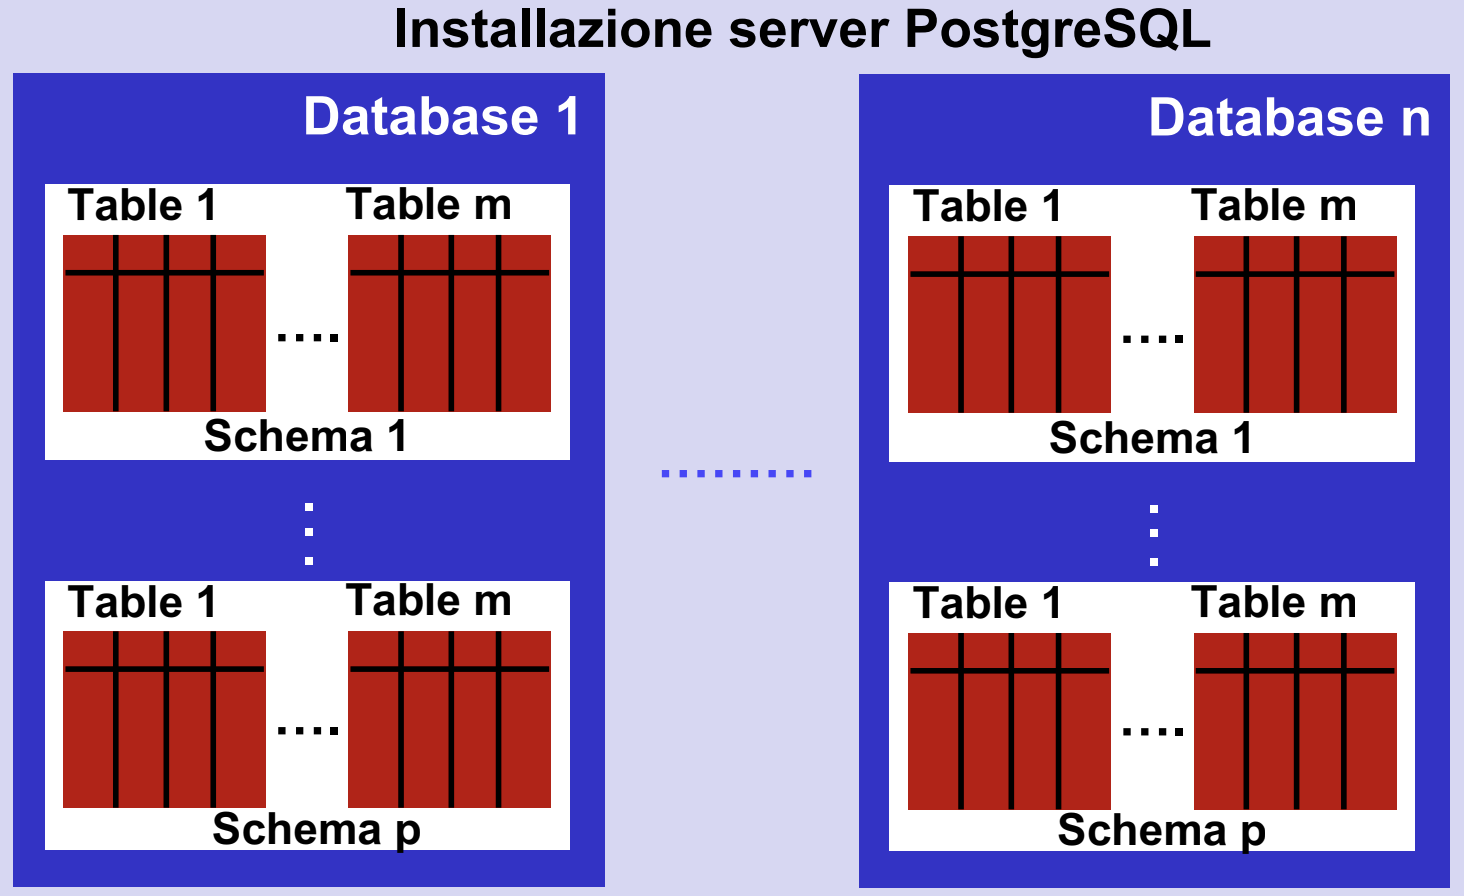
\includegraphics[width=0.7\linewidth]{../../images/database.png}
    %\caption{caption}
    %\label{label}
\end{figure}
\noindent Ogni utente si collega con un database, che si denota con Schema1.Table1 (oppure con solo Table1 se Schema1 è implicito), un utente connesso con Database1 "vede" tutti gli schemi di Database1 e nessuno schema di un altro Database. 
Un Database Postgres è una collezione di basi di dati, ognuno con il relativo schema e la relativa istanza.
\section{Istruzioni}
\begin{itemize}
    \item Ogni \textbf{tabella} si denota con \texttt{NomeSchema.NomeTabella}
    \item Ogni \textbf{attributo} di una tabella si denota con \texttt{NomeSchema.NomeTabella.Attributo}
\end{itemize}
Quando l'ambiguità sullo schema non sussiste si può omettere \texttt{NomeSchema.} e scrivere semplicemente \texttt{NomeTabella}\\
Quando l'ambiguità sullo schema non sussiste si può omettere \texttt{NomeSchema.} e scrivere \texttt{NomeTabella.Attributo}\\
Quando l'ambiguità sulla tabella non sussiste si può omettere \texttt{NomeTabella.} e scrivere semplicemente \texttt{Attributo}
\newpage 
\subsection{Select}
L'istruzione di interrogazione in SQL è \texttt{select} che definisce una interrogazione (query) e restituisce il risultato della valutazione di quella query sulla base di dati in forma di tabella. La sua forma elementare è:
\begin{verbatim}
    select  Attributo,...,Attributo
    from    Tabella
    where   Condizione
\end{verbatim}
\noindent semantica:\\
ogni tupla $t$ della Tabella è indicata nella clausola \underline{from} viene analizzata. Se $t$ non soddisfa la condizione nella clausola \underline{where}, allora viene ignorata. 
Altrimenti da $t$ viene prodotta la target list (lista attributi) secondo quanto specificato nella target list che appare dopo \underline{select} e la tupla risultante da tale target list viene inserita nel risultato. 
Il risultato della esecuzione della query viene restituito nel canale di output del sistema e volendo memorizzarlo nella base di dati.
La semantica descritta chiarisce che l'istruzione è analoga alla seguente espressione dell'algebra relazionale\\
$$PROJ_{Attributo,...,Attributo}(SEL_{Condizione}(Tabella))$$\\
Diciamo analoga e non equivalente perchè in sql la tabella può avere duplicati.\\
Esempio:
\begin{figure}[H]
    \centering  
    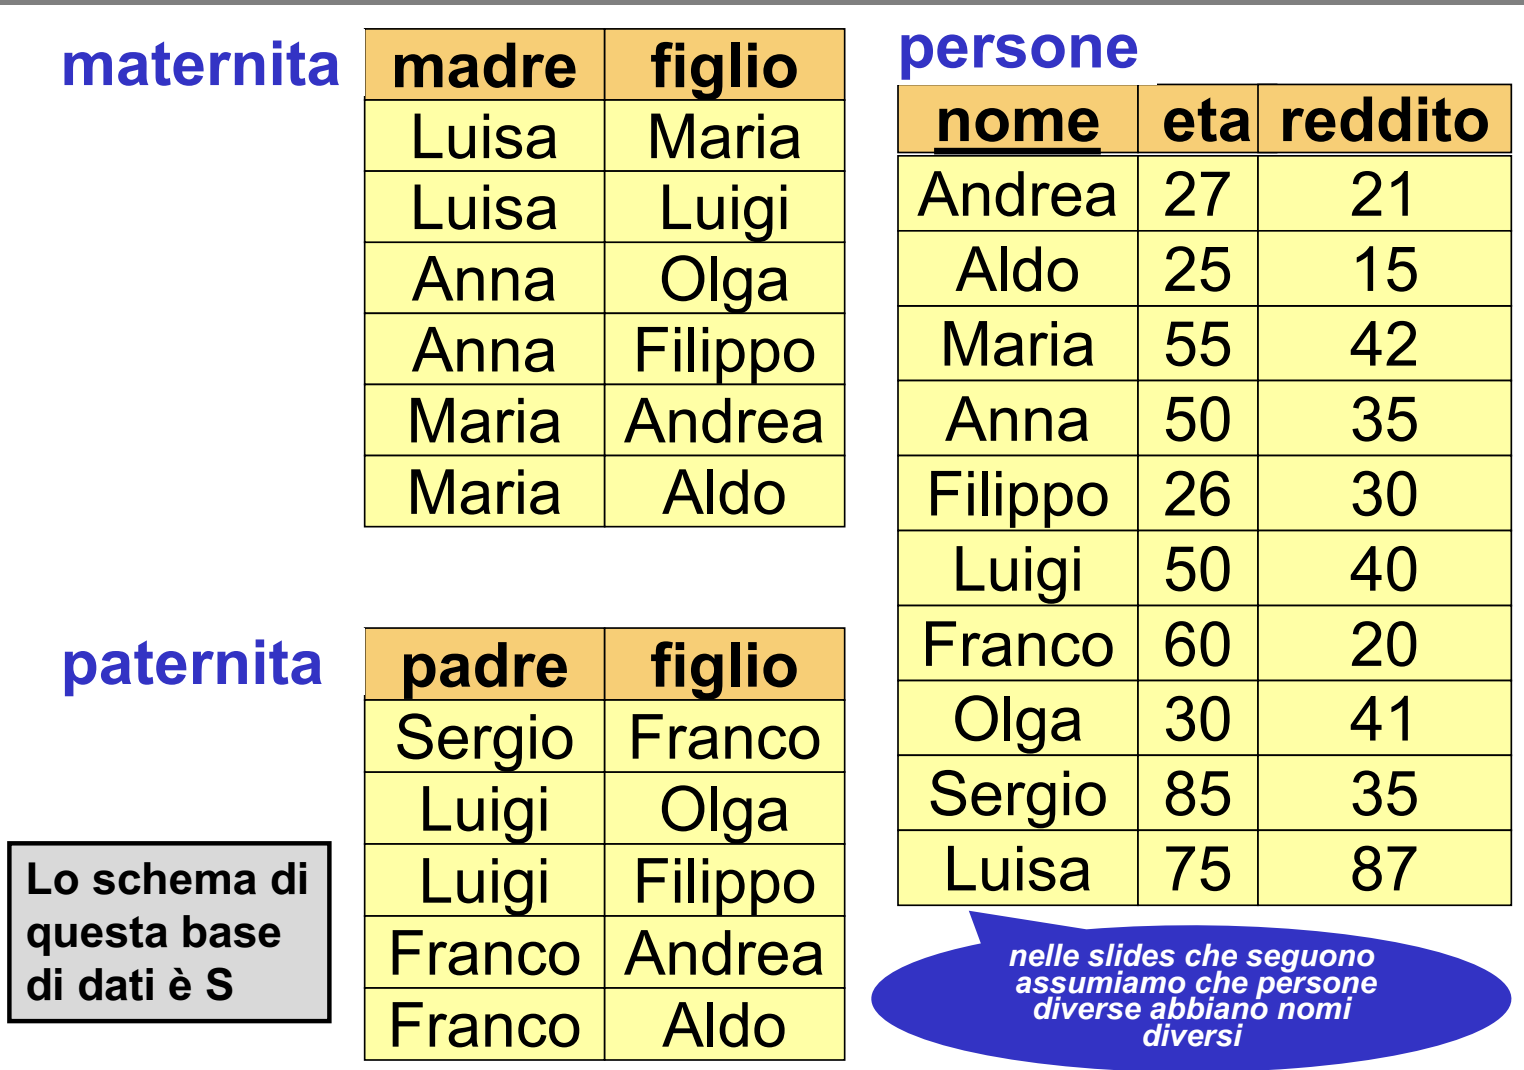
\includegraphics[width=0.7\linewidth]{../../images/sql1.png}
    %\caption{caption}
    %\label{label}
\end{figure}
\noindent Vogliamo il nome e reddito delle persone con meno di 30 anni.\\
$$PROJ_{nome,reddito}(SEL_{eta<30}(persone))$$
\begin{figure}[H]
    \centering
    \begin{minipage}[c]{0.70\textwidth}
       \begin{verbatim}
        select S.persone.nome, S.persone.reddito
        from S.persone
        where S.perone.eta<30
        \end{verbatim}
    \end{minipage}
    \hfill
    \begin{minipage}[c]{0.25\textwidth}
        \centering
        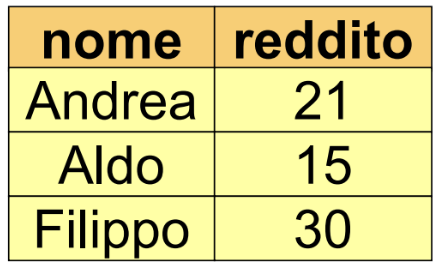
\includegraphics[width=0.8\linewidth]{../../images/sql2.png}
    \end{minipage}

    % \caption{caption}
    % \label{label}
\end{figure}
\noindent Da ora in poi assumiamo di essere nell'ambito dello schema S e quindi possiamo omettere il nome dello schema. In questo caso possiamo quindi scrivere:
\begin{verbatim}
    select persone.nome, persone.reddito
    from persone
    where persone.eta<30
\end{verbatim}
\noindent Nella query non c'è ambiguita su quali sono gli attributi: essi sono certamente quelli della tabella "persone" quindi la query si può scrivere:
\begin{verbatim}
    select nome, reddito
    from persone
    where eta<30
\end{verbatim}

\section{Ridenominazione As}
"as" nella lista degli attributi serve a ridenominare gli attributi, specificando esplicitamente un nome per un attributo del risultato.\\
Esempio:
\begin{verbatim}
select nome as name, reddito as salary
from persone
where eta<30
\end{verbatim}
\noindent restituisce com risultato una tabella con due attributi, il primo nome name ed il secondo salary.\\
"as" serve anche ad assegnare un nuovo nome alle tabelle nel'ambito di una query.\\
Esempio:
\begin{verbatim}
select p.nome as name, p.reddito as salary
from persone as p
where p.eta<30
\end{verbatim}
\section{Distinct, $<$, *, where, null}
\subsection{Distinct}
Per non avere duplicati nella query nella select aggiungiamo distinct\\
Esmepio:\\
\texttt{select distinct attributo1,...,attributo2 from tabella1}
\subsection{$<$}
La utilizziamo per evitare ridondanze quando stiamo confrontando righe della stessa tabella tra loro, tipicamente in un self join, e vogliamo ottenere ogni coppia una sola volta.\\
Esempio:
\begin{verbatim}
    select p1.nome, p2.nome
    from persona p1, persona p2
    where p1.id < p2.id
\end{verbatim}
\subsection{*}
Qunado vogliamo che una query restituisca tutti gli attributi usiamo '*' nella select al posto della lista degli attributi.\\
Esempio:\\
Data una tabella R sugli attributi A1,...,An:\medskip\\
\begin{minipage}[c]{0.40\textwidth}
       \begin{verbatim}
        select *
        from tabella1
        where condizione
        \end{verbatim}
    \end{minipage}
    equivale a
    \begin{minipage}[c]{0.25\textwidth}
        \begin{verbatim}
            select A1,...,An
            from R
            where condizione
        \end{verbatim}
\end{minipage}
\subsection{Condizione while}
Quando eseguiamo una query in cui non c'è una condizione possiamo scrivere while true o non scrivere proprio where.\\
Esempio:\\
\begin{minipage}[c]{0.40\textwidth}
       \begin{verbatim}
        select A1,...,An
        from tabella1
        \end{verbatim}
    \end{minipage}
    equivale a
    \begin{minipage}[c]{0.25\textwidth}
        \begin{verbatim}
            select A1,...,An
            from R
            where true
        \end{verbatim}
\end{minipage}\medskip\\
Nella clausola where possono comparire espressioni booleane qualunque\\
Esempio:\\
\texttt{select *
from persone
where reddito > 25 and (eta < 30 or eta >60)}\\
Nelle condizioni nella clausola where si possono usare molti operatori che SQL mette a disposizione.\\
Ad esempio l'operatore \texttt{like} che consente di verificare che una stringa appartenga al linguaggio definito da una espressione regolare.\\
Esempio:\\
se vogliamo conoscere quali sono le persone che hanno un nome che inizia per 'A', ha 'd' come terza lettera e può continuare con altri caratteri.
\begin{verbatim}
select *
from persone
where nome like 'A_d%'
\end{verbatim}
\subsection{gestione dei valori nulli - "is null" e "is not null"}
nelle condizioni che compaiono nella clausola where si possono usare anche i predicati "is null" e "is not null" per gestire i valori nulli\\
Esempio:\\
vogliamo le persone la cui eta è o ptrebbe essere maggiore di 40
\begin{verbatim}
select *
from persone
where eta > 40 or eta is null    
\end{verbatim}
\section{Espressioni nella target list}
Ogni elemento della target list può essere una espressione che fa uso dei valori memorizzati negli attributi delle tuple del risultato.\\
Esempio:\\
\texttt{select eta, reddito/2\\
from persone\\
where nome='Luigi'}\\
reddito/2 $\rightarrow$ espressione aritmetica che fa uso del valore dell'attributo reddito e lo divide per 2\\
Nella target list può comparire un numero qualunque di espressioni e all'interno di tali espressioni possono ovviamente comparire anche costanti\\
Esempio:\\
\texttt{select 'Gigi' as nomePersona, eta, reddito/2 as redditoSemestrale\\
from persone\\
where nome='Luigi'}\\
Espressione costituita da una costante di tipo stringa che aggiunge un attributo nomePersona con la stringa 'Gigi'\\
\begin{figure}[H]
    \centering  
    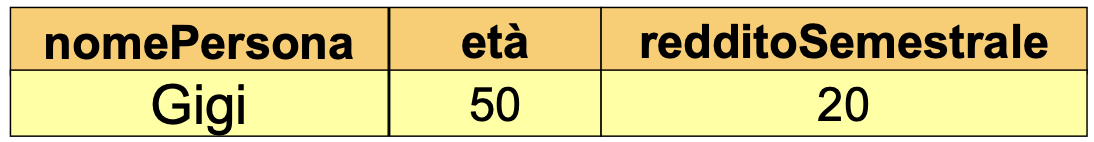
\includegraphics[width=0.5\linewidth]{../../images/query123.png}
    %\caption{caption}
    %\label{label}
\end{figure}

\section{Selezione, proiezione e join}
le istruzioni select che abbiamo visto finora hanno una sola tabella nella clausola from e quindi permettono di realizzare:
\begin{itemize}
    \item selezioni
    \item proiezioni
    \item ridenominazioni
\end{itemize}
\noindent I joni si possono realizzare indicando due o più tabelle nella clausola from, separate da virgola
\subsection{Select}
\subsubsection{sintassi e semantica}
La forma base delle selct in SQL è:
\begin{verbatim}
    select <target list>  --> lista attributi
    from R1,R2,...,Rn
    where <condizione>
\end{verbatim}
\noindent In algebra relazionale: $PROJ_{target list}(SEL_{<condizione>}(R_1 \times R_2 \times ... \times R_n))$\\
Ogni tupla t del prodotto cartesiano viene analizzata. Se t non verifica la condizione della clausola WHERE, essa viene ignorata. Se invece t verifica la condizione della clausola 
WHERE, allora da t viene prodotta la target list secondo la proiezione specificata nella clausola SELECT e la tupla risultante da tale target list viene inserita nel risultato\\
\underline{Attenzione}: questo non significa che il DBMS calcola il prodotto cartesiano di R1,R2,..,Rn. Significa che ilrisultato ottenuto è lo stesso di quello che si ottiene partendo dal prodotto cartesiano.
\subsection{Join}
Date due relazioni: R1(A1, A2) e R2(A3, A4)
\begin{verbatim}
    select R1.A1, R2.A4
    from R1, R2
    where R1.A2 = R2.A3
\end{verbatim}
\noindent è analoga a: $PROJ_{A1,A4}(R1 \text{ }JOIN_{A2=A3}\text{ }R2)$\\
Possono essere necessarie ridenominazioni:
\begin{itemize}
    \item nella target list
    \item nella clausola from (in particolare, introdurre alias consente di riferirsi due o più volte alla stessa tabella)
\end{itemize}
\noindent Esempio:
\begin{verbatim}
    select X.A1 as B1,...
    from R1 as X, R2 as Y, R1 as Z
    where X.A2 = Y.A3 and Y.A4 = Z.A1
\end{verbatim}
\noindent Si può anche scireve senza 'as'.\medskip\\
Date le tabelle R1(A1, A2) e R2(A3, A4)
\begin{verbatim}
    select distinct X.A1 as B1, Y.A4 as B2
    from R1 as X, R2 as Y, R1 as Z
    where X.A2 = Y.A3 and Y.A4 = Z.A1 
\end{verbatim}
\noindent è equivalente a:
$REN_{B1,B2 \leftarrow A1,A4}( PROJ_{A1,A4} (SEL_{A2=A3 \text{ and }A4=C1 }( R1 \text{ }JOIN\text{ }R2\text{ }JOIN\text{ }REN_{C1,C2 \leftarrow A1,A2}(R1))))$
\subsection{Self-join}
Il self-join è un join in cui la stessa relazione compare sia come operando sinistro sia come operando destro ed è cruciale quando dobbiamo combinare due tuple della stessa relazione.\\
Esempio:\\
\texttt{persone(nome, eta, reddito)}\\
\underline{query}: Vogliamo le coppie di persone con lo stesso reddito\\
\underline{soluzione}:
\begin{verbatim}
    select p1.nome, p1.eta, p1.reddito, p2.nome, p2.eta
    from persone p1, persone p2
    where p1.reddito=p2.reddito and p1.nome<p2.nome
\end{verbatim}
\noindent utilizziamo p1.nome $<$ p2.nome per eliminare le tuple ridondanti, in quando lascia solo le tuple in cui p1.nome viene prima in ordine alfabetico di p2.nome

\subsection{Join multipli}

Quando una query richiede di mettere in relazione informazioni provenienti da più tabelle, è possibile eseguire \textbf{più join nella stessa interrogazione}. L'idea è costruire progressivamente il risultato: ogni join collega una nuova tabella al risultato ottenuto dai join precedenti attraverso una specifica condizione.
Un primo esempio riguarda la ricerca del \textbf{padre e della madre di ogni persona della quale entrambi i genitori sono noti}. Le tabelle \texttt{paternita} e \texttt{maternita} possiedono entrambe l'attributo \texttt{figlio}, che permette di collegare le informazioni relative alla stessa persona:

\begin{verbatim}
select paternita.figlio, padre, madre
from maternita, paternita
where paternita.figlio = maternita.figlio
\end{verbatim}

\noindent In questo caso è sufficiente un solo join. Se, però, si vuole anche garantire che il figlio compaia effettivamente nella tabella \texttt{persone}, è necessario introdurre un \textbf{secondo join}:

\begin{verbatim}
select paternita.figlio, padre, madre
from maternita, paternita, persone
where paternita.figlio = maternita.figlio
  and paternita.figlio = persone.nome
\end{verbatim}

\noindent Quindi, quando sono presenti più join, nella clausola \texttt{from} vengono indicate tutte le tabelle coinvolte, mentre nella clausola \texttt{where} vengono specificate le condizioni che stabiliscono come collegarle tra loro. Ogni condizione di join permette di associare tuple che rappresentano entità correlate. 
Un caso più articolato si presenta quando la \textbf{stessa tabella deve essere utilizzata più volte con ruoli differenti}. L'esempio considerato è quello delle persone che guadagnano più dei rispettivi padri, mostrando il nome della persona, il suo reddito e il reddito del padre.
La tabella \texttt{persone} deve comparire due volte: una volta per rappresentare il \textbf{padre} e una volta per rappresentare il \textbf{figlio}. Per distinguere le due occorrenze si utilizzano degli \textbf{alias}:

\begin{verbatim}
select f.nome, f.reddito as reddito,
       p.reddito as redditoPadre
from persone p, paternita t, persone f
where p.nome = t.padre
  and t.figlio = f.nome
  and f.reddito > p.reddito
\end{verbatim}

\noindent Gli alias hanno quindi un ruolo fondamentale:
\begin{itemize}
    \item \texttt{p} rappresenta la persona nel ruolo di \textbf{padre};
    \item \texttt{t} rappresenta la tabella \texttt{paternita};
    \item \texttt{f} rappresenta la persona nel ruolo di \textbf{figlio}.
\end{itemize}

\noindent I join vengono concettualmente costruiti in più passaggi. Prima si collega \texttt{paternita} alla copia di \texttt{persone} che rappresenta il figlio, mediante la corrispondenza

\[
\texttt{t.figlio = f.nome}.
\]

\noindent In questo modo si ottengono insieme le informazioni sulla relazione di paternità e quelle relative al figlio. Successivamente si collega anche la copia di \texttt{persone} che rappresenta il padre:

\[
\texttt{p.nome = t.padre}.
\]

\noindent A questo punto ogni tupla contiene le informazioni necessarie sia sul figlio sia sul relativo padre. È quindi possibile applicare la condizione

\[
\texttt{f.reddito > p.reddito},
\]

\noindent che mantiene solamente i casi in cui il reddito del figlio è maggiore di quello del padre. Infine, con la \texttt{select} vengono mantenuti solamente gli attributi richiesti: nome del figlio, reddito del figlio e reddito del padre.
In generale, quindi, una query con \textbf{più join} può essere vista come una costruzione progressiva: si collegano prima due tabelle, il risultato viene poi collegato a un'altra tabella e così via. Se una stessa tabella deve rappresentare entità con ruoli differenti, la si inserisce più volte nella query assegnandole alias diversi. Le condizioni nella clausola \texttt{where} stabiliscono sia i collegamenti tra le varie occorrenze delle tabelle sia gli eventuali ulteriori criteri di selezione.

\subsection{Join esplicito}
\begin{verbatim}
select ...
from Tabella1 join Tabella2 on CondJoin,...
[where AltraCondizione]
\end{verbatim}

\noindent La parola chiave \texttt{join} specifica le tabelle da combinare, mentre la clausola \texttt{on} contiene la \textbf{condizione di join}, cioè la condizione che stabilisce quali tuple delle due tabelle devono essere associate. La clausola \texttt{where}, invece, può essere utilizzata per imporre ulteriori condizioni sul risultato del join.\\
Ad esempio, per ottenere padre e madre delle persone per le quali entrambi i genitori sono noti, invece di scrivere:
\begin{verbatim}
select paternita.figlio, padre, madre
from maternita, paternita
where paternita.figlio = maternita.figlio
\end{verbatim}
\noindent si può utilizzare il join esplicito:
\begin{verbatim}
select madre, paternita.figlio, padre
from maternita join paternita on
     paternita.figlio = maternita.figlio
\end{verbatim}
\noindent In questo caso si tratta di un \textbf{equi-join}, perché la condizione specificata dopo \texttt{on} è un'uguaglianza.
Il join esplicito può essere applicato \textbf{più volte consecutivamente}. Il risultato di un primo join è infatti una nuova tabella, che può essere utilizzata come operando di un secondo join. Ad esempio:
\begin{verbatim}
select f.nome, f.reddito, p.reddito
from persone p
     join paternita t on p.nome = t.padre
     join persone f on t.figlio = f.nome
where f.reddito > p.reddito
\end{verbatim}
\noindent Il primo join:
\begin{verbatim}
persone p join paternita t on p.nome = t.padre
\end{verbatim}
\noindent collega ogni padre alla relativa informazione nella tabella \texttt{paternita}. Il risultato viene poi utilizzato nel secondo join:
\begin{verbatim}
join persone f on t.figlio = f.nome
\end{verbatim}
\noindent che associa anche le informazioni relative al figlio. Solo dopo aver costruito questi collegamenti viene applicata la condizione:
\begin{verbatim}
where f.reddito > p.reddito
\end{verbatim}
\noindent per mantenere i figli che guadagnano più del rispettivo padre.
È importante osservare che il \textbf{risultato di un join contiene gli attributi di entrambi gli operandi}. Di conseguenza, se si eseguono più join consecutivi, ogni risultato intermedio accumula gli attributi delle tabelle coinvolte.
Nella query sopra, il primo join esplicito nella clausola fromdà come risultato
una tabella con gli attributi: \texttt{p.nome, p.eta, p.reddito, t.padre. t.figlio}. Questa
tabella va in input al secondo join esplicito il cui risultato avrà come attributi:
\texttt{p.nome, p.eta, p.reddito, t.padre. t.figlio, f.nome, f.eta, ed f.reddito}.\\
In sintesi, il join esplicito permette di separare chiaramente le \textbf{condizioni che servono a collegare le tabelle}, scritte nella clausola \texttt{on}, dalle \textbf{condizioni che servono a filtrare il risultato}, che possono essere scritte nella clausola \texttt{where}. Inoltre, più join possono essere concatenati, utilizzando ogni risultato intermedio come operando del join successivo.
\subsection{Ridenominazione del risultato di un join esplicito}
Poiché il risultato di un join esplicito è una \textbf{tabella}, esso può essere utilizzato direttamente nella clausola \texttt{from} e può anche essere \textbf{ridenominato assegnandogli un alias}.
Riprendiamo l'esempio precedente. Il primo join era:
\begin{verbatim}
persone p join paternita t on p.nome = t.padre
\end{verbatim}
\noindent Questo join produce una tabella contenente gli attributi di entrambi gli operandi:
\[
p.nome,\ p.eta,\ p.reddito,\ t.padre,\ t.figlio.
\]
\noindent È possibile assegnare un alias, ad esempio \texttt{J}, all'intero risultato del join:
\begin{verbatim}
from (persone p join paternita t on p.nome = t.padre) as J,
     persone f
\end{verbatim}
\noindent Quando si assegna un alias a un join esplicito è necessario \textbf{racchiudere tra parentesi l'intera espressione di join}.
Un aspetto importante è la \textbf{visibilità degli alias}. Gli alias \texttt{p} e \texttt{t}, definiti all'interno delle parentesi, non sono più
referenziabili all'esterno. All'esterno delle parentesi è visibile solamente l'alias \texttt{J}.
Di conseguenza, invece di riferirsi agli attributi attraverso \texttt{p} e \texttt{t}, bisogna utilizzare \texttt{J}. Ad esempio:
\begin{verbatim}
where f.reddito > J.reddito
  and f.nome = J.figlio
\end{verbatim}
\noindent In questo caso:
\[
\texttt{J.reddito}
\]

\noindent indica l'attributo \texttt{reddito} proveniente dalla tabella \texttt{persone p}, mentre
\[
\texttt{J.figlio}
\]

\noindent indica l'attributo \texttt{figlio} proveniente dalla tabella \texttt{paternita t}. La query può quindi essere scritta come:
\begin{verbatim}
select f.nome, f.reddito, J.reddito
from (persone p join paternita t on p.nome = t.padre) as J,
     persone f
where f.reddito > J.reddito
  and f.nome = J.figlio
\end{verbatim}
\noindent L'alias \texttt{J} deve quindi essere visto come il \textbf{nome della nuova tabella prodotta dal join}, che eredita gli attributi delle tabelle utilizzate
per costruirla.

\subsection{Ridenominazione degli attributi del risultato}
Quando la struttura dei join diventa più complessa, assegnare soltanto un nome
al risultato può non essere sufficiente. SQL permette quindi di specificare,
oltre al nome della nuova tabella, anche i \textbf{nomi dei suoi attributi}.\medskip\\
Ricordando che il database è così composto:\\
\texttt{
persone(nome, eta, reddito): contiene le informazioni sulle persone.\\
paternita(padre, figlio): rappresenta le relazioni padre-figlio.\\
maternita(madre, figlio): rappresenta le relazioni madre-figlio.\\
}\\
\noindent Supponiamo ora di volere le coppie (senza ridondanze) di persone diverse
che hanno la stessa età e sono figli dello stesso padre.
Vogliamo utilizzare un join tra due join espliciti, uno per individuare le coppie
di persone diverse con la stessa eta (alias F) e l’altro per individuare le
coppie di tuple di paternita con lo stesso valore per “figlio".
Consideriamo un join tra due occorrenze della tabella \texttt{persone}:
\begin{verbatim}
persone r join persone s
on r.eta = s.eta and r.nome < s.nome
\end{verbatim}

\noindent Il risultato possiede sei attributi, cioè i tre attributi di \texttt{r} seguiti
dai tre attributi di \texttt{s}. Possiamo ridenominare l'intero risultato e,
contemporaneamente, i suoi attributi:
\begin{verbatim}
(persone r join persone s
 on r.eta = s.eta and r.nome < s.nome)
as F(n1,e1,r1,n2,e2,r2)
\end{verbatim}

\noindent L'alias non è quindi più soltanto \texttt{F}, ma specifica anche lo schema
della tabella risultante:
\[
F(n1,e1,r1,n2,e2,r2).
\]

\noindent I nomi vengono assegnati agli attributi rispettando il loro ordine. Quindi,
ad esempio, il primo attributo \texttt{r.nome} diventa \texttt{F.n1}, mentre
\texttt{s.nome} diventa \texttt{F.n2}.
Lo stesso meccanismo può essere applicato a un altro join:
\begin{verbatim}
(paternita p join paternita t on p.padre = t.padre)
as S(p1,f1,p2,f2)
\end{verbatim}

\noindent A questo punto i risultati dei due join possiedono attributi con nomi
esplicitamente definiti e possono essere a loro volta messi in join:
\begin{verbatim}
select F.n1, F.n2
from (persone r join persone s
      on r.eta = s.eta and r.nome < s.nome)
     as F(n1,e1,r1,n2,e2,r2)
join
     (paternita p join paternita t
      on p.padre = t.padre)
     as S(p1,f1,p2,f2)
on F.n1 = S.f1 and F.n2 = S.f2
\end{verbatim}

\noindent La ridenominazione degli attributi permette quindi di utilizzare senza ambiguità gli attributi dei \textbf{risultati intermedi dei join}, anche
quando si costruisce un join tra risultati di altri join espliciti.



\noindent da 60 fino a pagina 128 sql\\
pagina 148 slide modello relazionale fino a 160